\documentclass{article}
\usepackage[paperwidth=360pt,paperheight=230pt,margin=0pt,noheadfoot]{geometry}
\usepackage{tikz}
\usetikzlibrary{calc}

\definecolor{ink}{RGB}{28,41,56}
\definecolor{axis}{RGB}{100,116,139}
\definecolor{grid}{RGB}{203,213,225}
\definecolor{curve}{RGB}{30,64,175}
\definecolor{teal}{RGB}{13,148,136}
\definecolor{tealfill}{RGB}{176,227,219}
% Integral diagrams use exactly one semantic palette: blue for the
% lower-only part, yellow for the upper-only (or still unresolved) part, and
% green for their common part.  The common part is explicit rather than an
% alpha blend, so the three meanings stay distinct after GIF quantization.
\definecolor{blue}{RGB}{0,114,178}
\definecolor{bluefill}{RGB}{86,180,233}
\definecolor{yellow}{RGB}{230,159,0}
\definecolor{yellowfill}{RGB}{255,218,102}
\definecolor{green}{RGB}{0,128,84}
\definecolor{greenfill}{RGB}{89,190,142}
\definecolor{orange}{RGB}{234,88,12}
\definecolor{orangefill}{RGB}{254,215,170}
\definecolor{purple}{RGB}{126,34,206}
\definecolor{yellowedge}{RGB}{202,138,4}
\definecolor{projection}{RGB}{148,163,184}
\colorlet{under}{blue}
\colorlet{underfill}{bluefill}
\colorlet{over}{yellow}
\colorlet{overfill}{yellowfill}
\colorlet{shared}{green}
\colorlet{sharedfill}{greenfill}
\colorlet{gap}{yellow}
\colorlet{gapfill}{yellowfill}

\pagestyle{empty}
\setlength\parindent{0pt}
\setlength\topskip{0pt}
\begin{document}
\noindent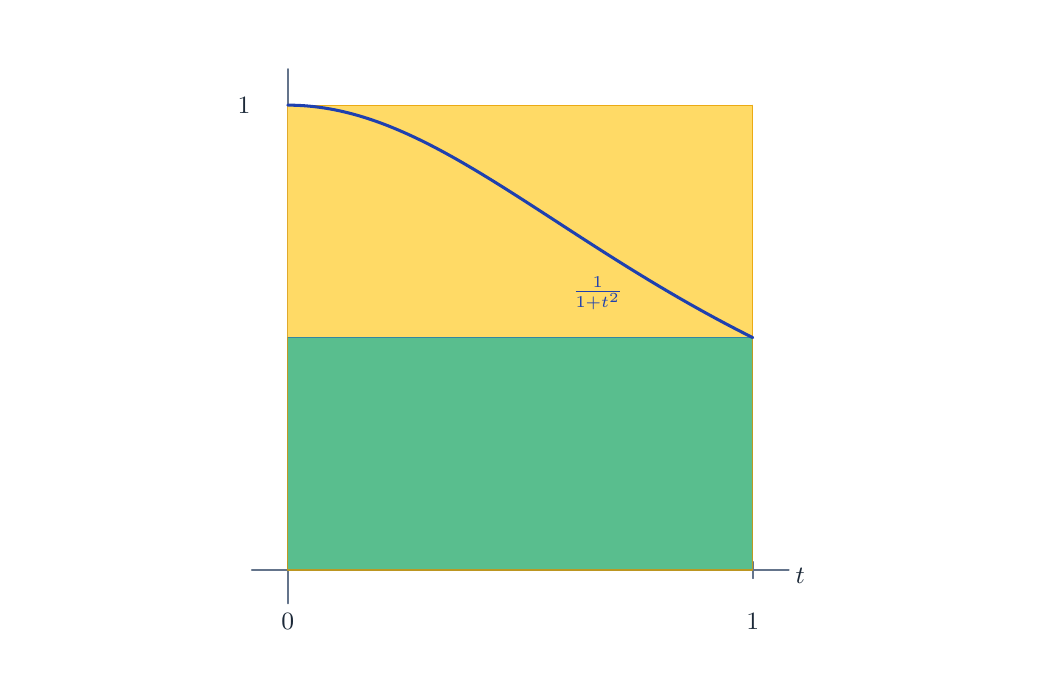
\begin{tikzpicture}[baseline=(current bounding box.north),x=1pt,y=1pt,line cap=round,line join=round]
\useasboundingbox (0,0) rectangle (360,230);
\draw[axis,line width=.75pt] (81,34) -- (275,34);
\draw[axis,line width=.75pt] (94,22) -- (94,215);
\draw[grid,line width=.3pt] (94,34) -- (94,202);
\draw[axis,line width=.55pt] (94,31) -- (94,37);
\draw[grid,line width=.3pt] (262,34) -- (262,202);
\draw[axis,line width=.55pt] (262,31) -- (262,37);
\path[fill=sharedfill] (94,34) rectangle (262,118);
\path[fill=overfill] (94,118) rectangle (262,202);
\draw[under,draw opacity=.8,line width=0.45pt] (94,34) rectangle (262,118);
\draw[over,draw opacity=.8,line width=0.45pt] (94,34) rectangle (262,202);
\draw[curve,line width=1.1pt] plot[smooth] coordinates {(94,202) (95.68,201.9832) (97.36,201.9328) (99.04,201.8489) (100.72,201.7316) (102.4,201.581) (104.08,201.3974) (105.76,201.1808) (107.44,200.9316) (109.12,200.6501) (110.8,200.3366) (112.48,199.9915) (114.16,199.6151) (115.84,199.208) (117.52,198.7705) (119.2,198.3032) (120.88,197.8066) (122.56,197.2812) (124.24,196.7276) (125.92,196.1465) (127.6,195.5385) (129.28,194.9041) (130.96,194.2442) (132.64,193.5593) (134.32,192.8502) (136,192.1176) (137.68,191.3623) (139.36,190.585) (141.04,189.7864) (142.72,188.9673) (144.4,188.1284) (146.08,187.2707) (147.76,186.3948) (149.44,185.5015) (151.12,184.5916) (152.8,183.6659) (154.48,182.7252) (156.16,181.7703) (157.84,180.8018) (159.52,179.8207) (161.2,178.8276) (162.88,177.8233) (164.56,176.8086) (166.24,175.7841) (167.92,174.7507) (169.6,173.7089) (171.28,172.6596) (172.96,171.6034) (174.64,170.541) (176.32,169.4729) (178,168.4) (179.68,167.3228) (181.36,166.2418) (183.04,165.1578) (184.72,164.0712) (186.4,162.9827) (188.08,161.8928) (189.76,160.802) (191.44,159.7109) (193.12,158.6198) (194.8,157.5294) (196.48,156.4401) (198.16,155.3522) (199.84,154.2663) (201.52,153.1827) (203.2,152.1019) (204.88,151.0242) (206.56,149.95) (208.24,148.8796) (209.92,147.8134) (211.6,146.7517) (213.28,145.6947) (214.96,144.6428) (216.64,143.5962) (218.32,142.5552) (220,141.52) (221.68,140.4909) (223.36,139.468) (225.04,138.4516) (226.72,137.4419) (228.4,136.439) (230.08,135.4431) (231.76,134.4544) (233.44,133.473) (235.12,132.4991) (236.8,131.5327) (238.48,130.5739) (240.16,129.623) (241.84,128.6799) (243.52,127.7448) (245.2,126.8177) (246.88,125.8987) (248.56,124.9879) (250.24,124.0853) (251.92,123.1909) (253.6,122.3049) (255.28,121.4271) (256.96,120.5578) (258.64,119.6968) (260.32,118.8442) (262,118)};
\node[font=\small,text=ink,anchor=north] at (94,22) {$0$};
\node[font=\small,text=ink,anchor=north] at (262,22) {$1$};
\node[font=\small,text=ink,anchor=east] at (84,202) {$1$};
\node[font=\small,text=ink,anchor=west] at (274,32) {$t$};
\node[font=\small,text=ink,text=curve] at (206,134) {$\frac{1}{1+t^2}$};
\end{tikzpicture}
\end{document}
